% Snowmass nEDM experimental status
\begin{figure}[p]
    \centering
    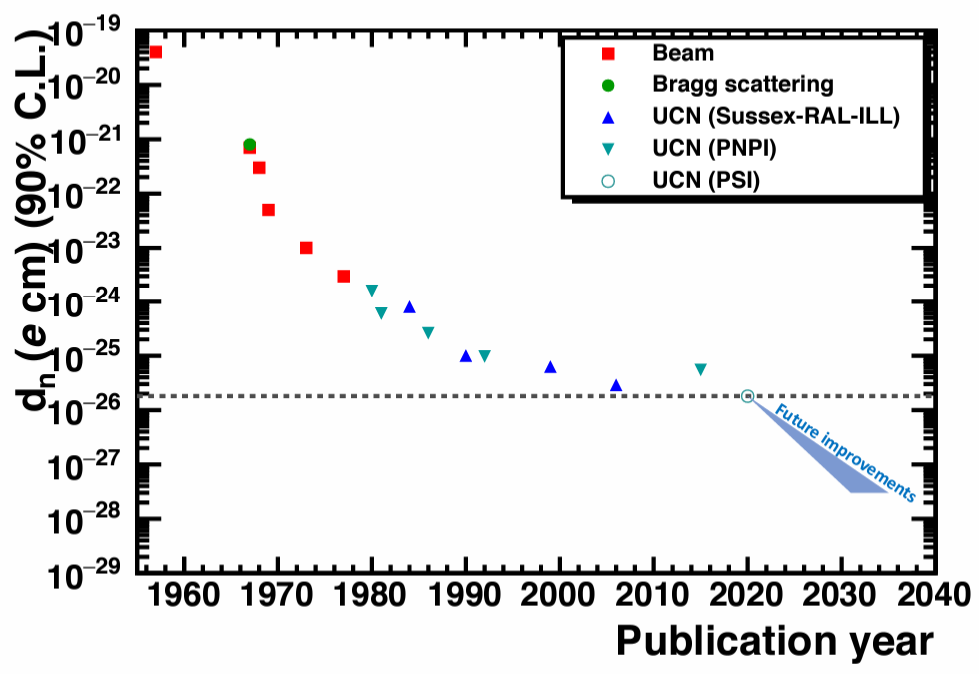
\includegraphics[width=0.7\linewidth]{Snowmass_fig.png}
    \caption{nEDM experimental progress~\cite{Snowmass2022EDM}}
    \label{fig:snowmass}
\end{figure}

% nEDM fixed rho_uu
\begin{figure}[p]
    \centering
    % \includegraphics[width=0.7\linewidth]{example-image}
    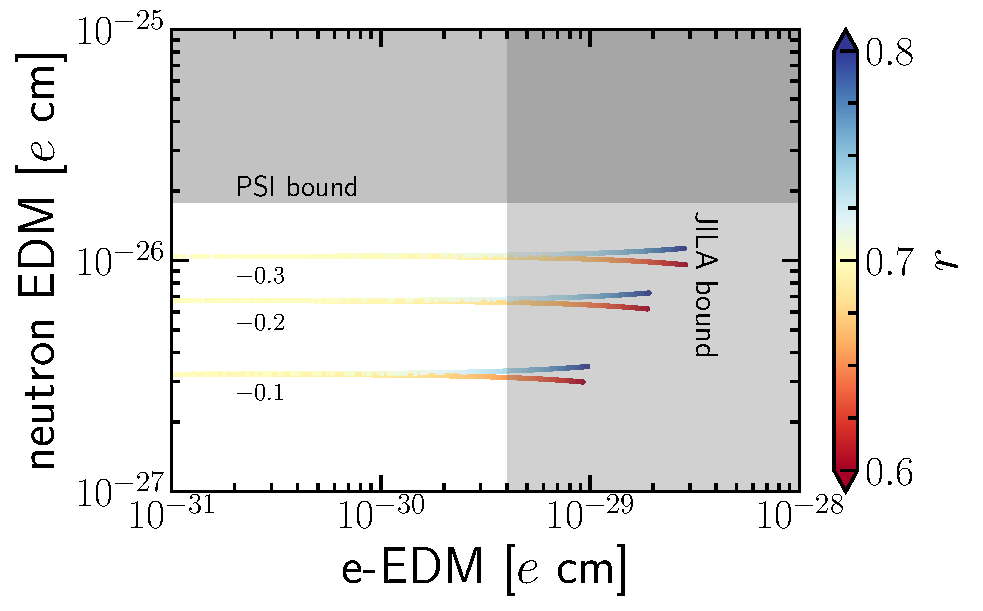
\includegraphics[width=0.8\linewidth]{fig3.pdf}
    \caption{nEDM results with extended ansatz.}
    \label{fig:nEDM-fixed}
\end{figure}

% % Combined nEDM-eEDM fixed rho_uu
% \begin{figure}[p]
%   \centering
%   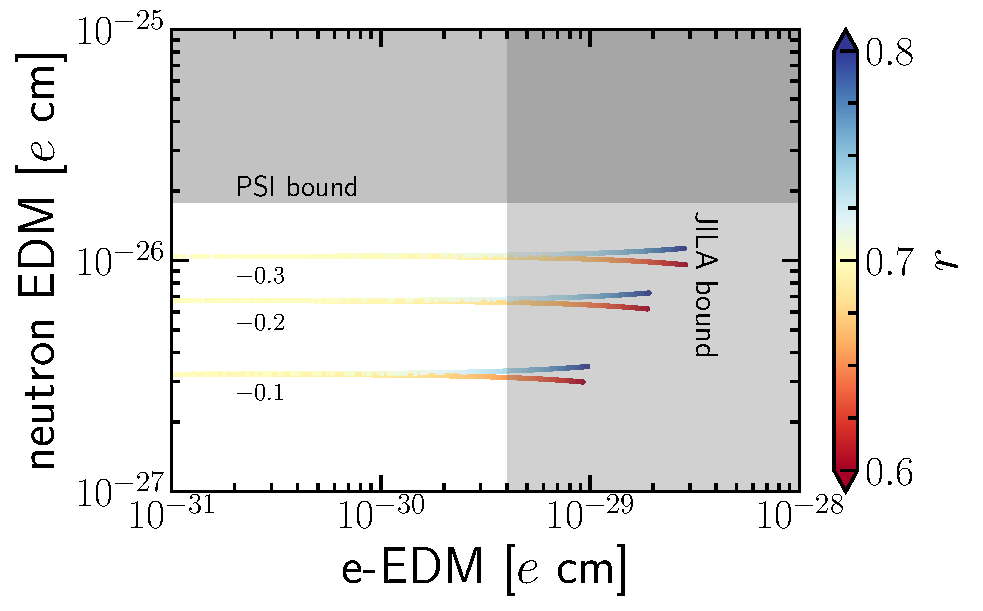
\includegraphics[width=0.95\linewidth]{fig3.pdf}
%   \caption{Combined eEDM-nEDM results.}
%   \label{fig:nEDM-eEDM}
% \end{figure}

% nEDM varying rho_uu
\begin{figure}[p]
    \centering
    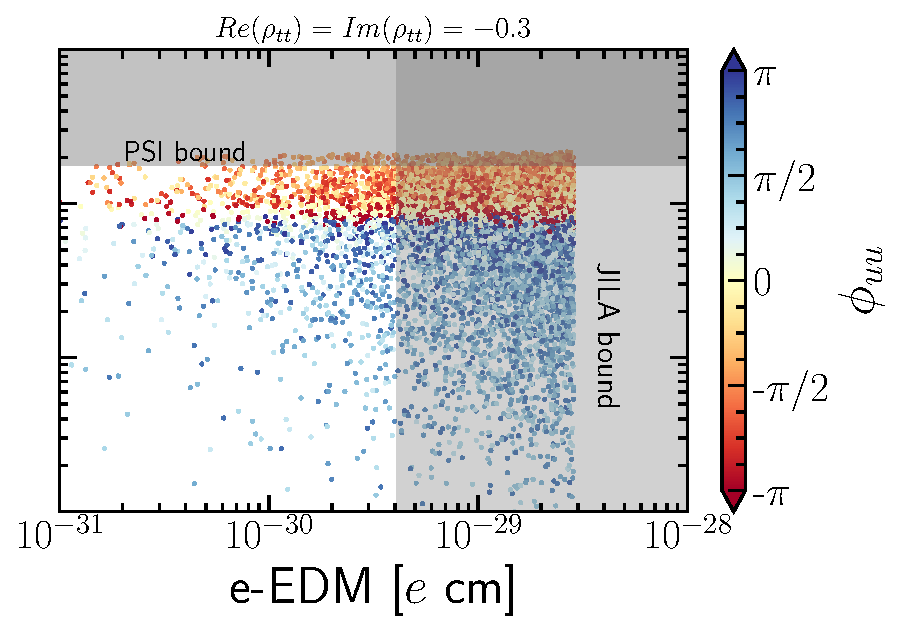
\includegraphics[width=7.89cm,height=5.55cm,angle=90]{fig4_3.pdf}\\
    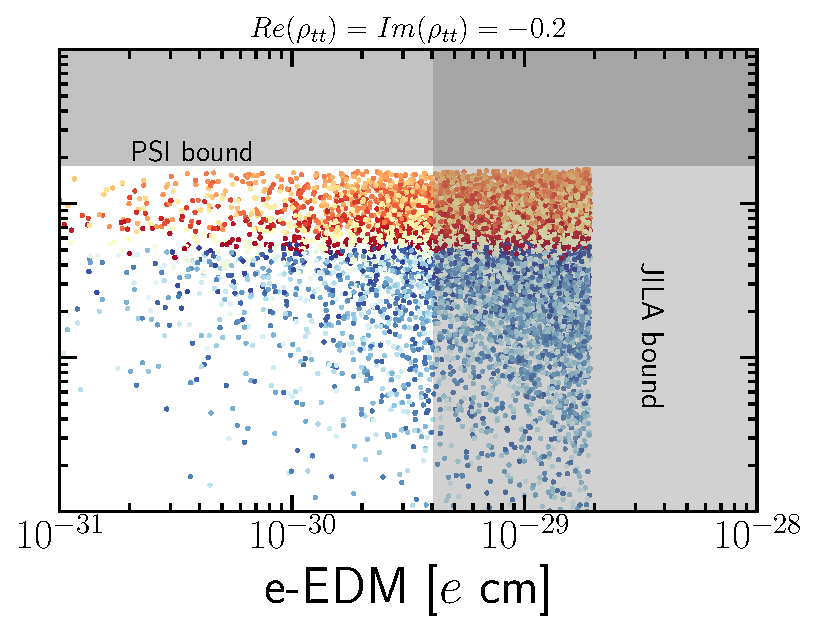
\includegraphics[width=6.45cm,height=5.55cm,angle=90]{fig4_2.pdf}\\
    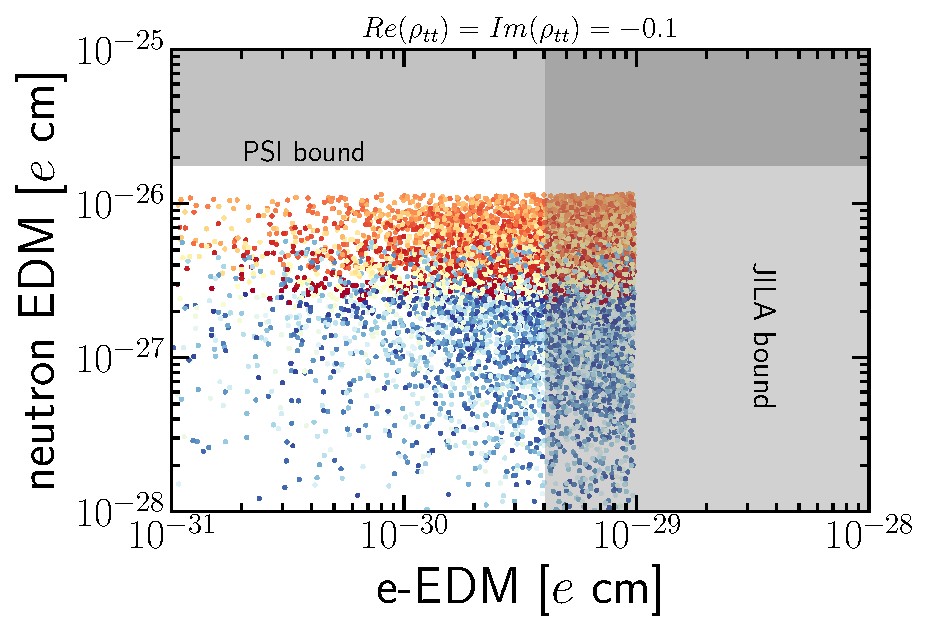
\includegraphics[width=7.35cm,height=5.55cm,angle=90]{fig4_1.pdf}
    \caption{Results for eEDM and nEDM with \(|\rho_{uu}| \sim \lambda_{u}\).}
    \label{fig:nEDM-varied}
\end{figure}